\subsection{Taxi event distribution}
\label{section_taxi_denstiy_distribution}

To validate $assumption 2$, we quantitatively analyze vehicles density in one hour. By dividing the whole network into $100*100$ grids, taxi density distributions for event 0, 1 are computed in each cell.

\begin{figure*}
\centering
\subfigure[$on-event,7:00-8:00$]{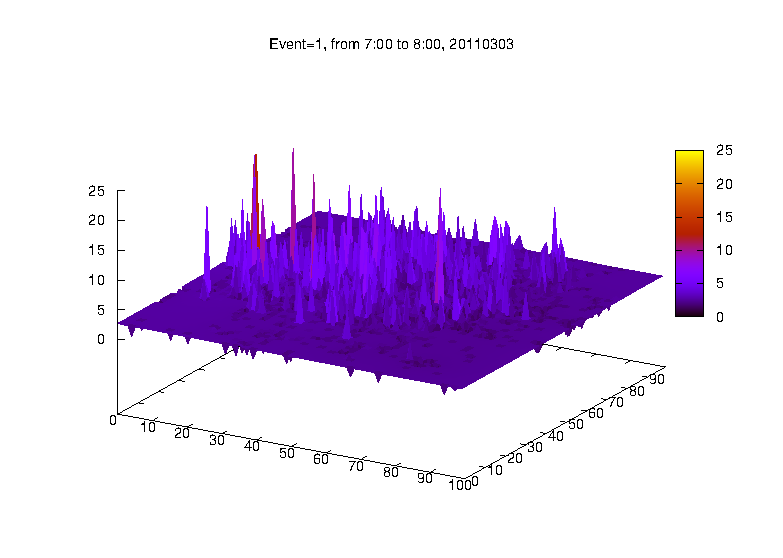
\includegraphics[width=0.3\textwidth]{figures_201103/events_dis/Event=1_7_8_20110303.eps}}
\subfigure[$on-event,12:00-13:00$]{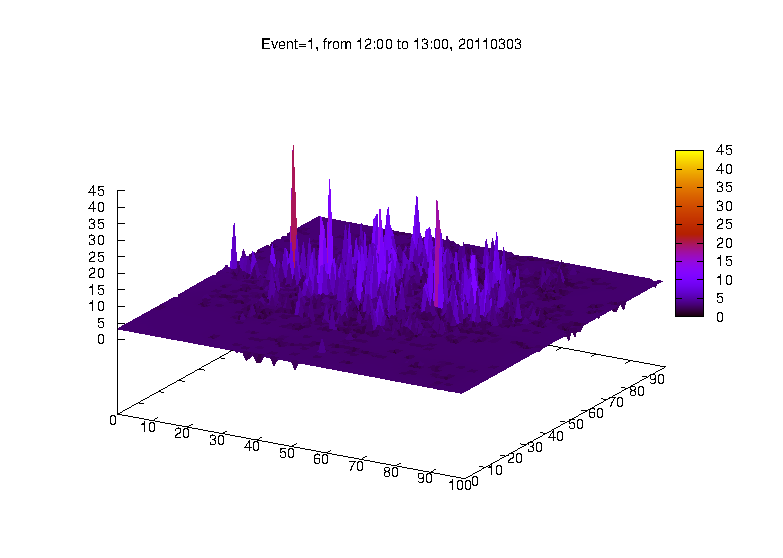
\includegraphics[width=0.3\textwidth]{figures_201103/events_dis/Event=1_12_13_20110303.eps}}
\subfigure[$on-event,17:00-18:00$]{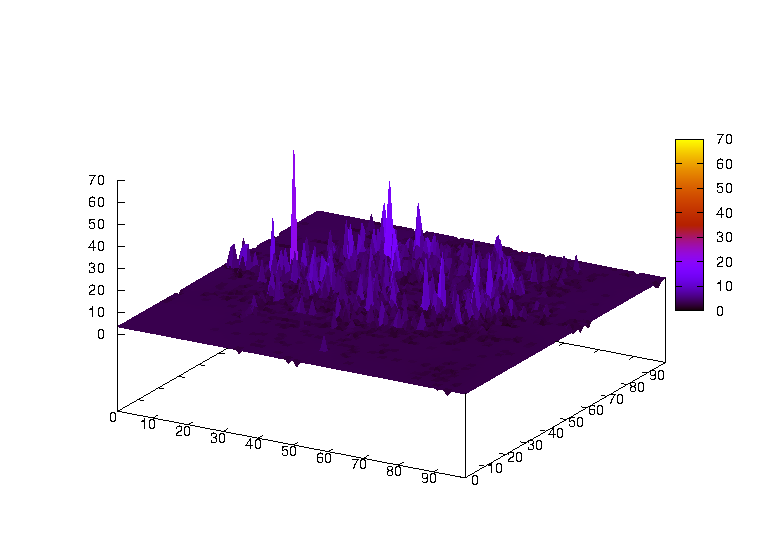
\includegraphics[width=0.3\textwidth]{figures_201103/events_dis/Event=1_17_18_20110303.eps}}
\subfigure[$off-event,7:00-8:00$]{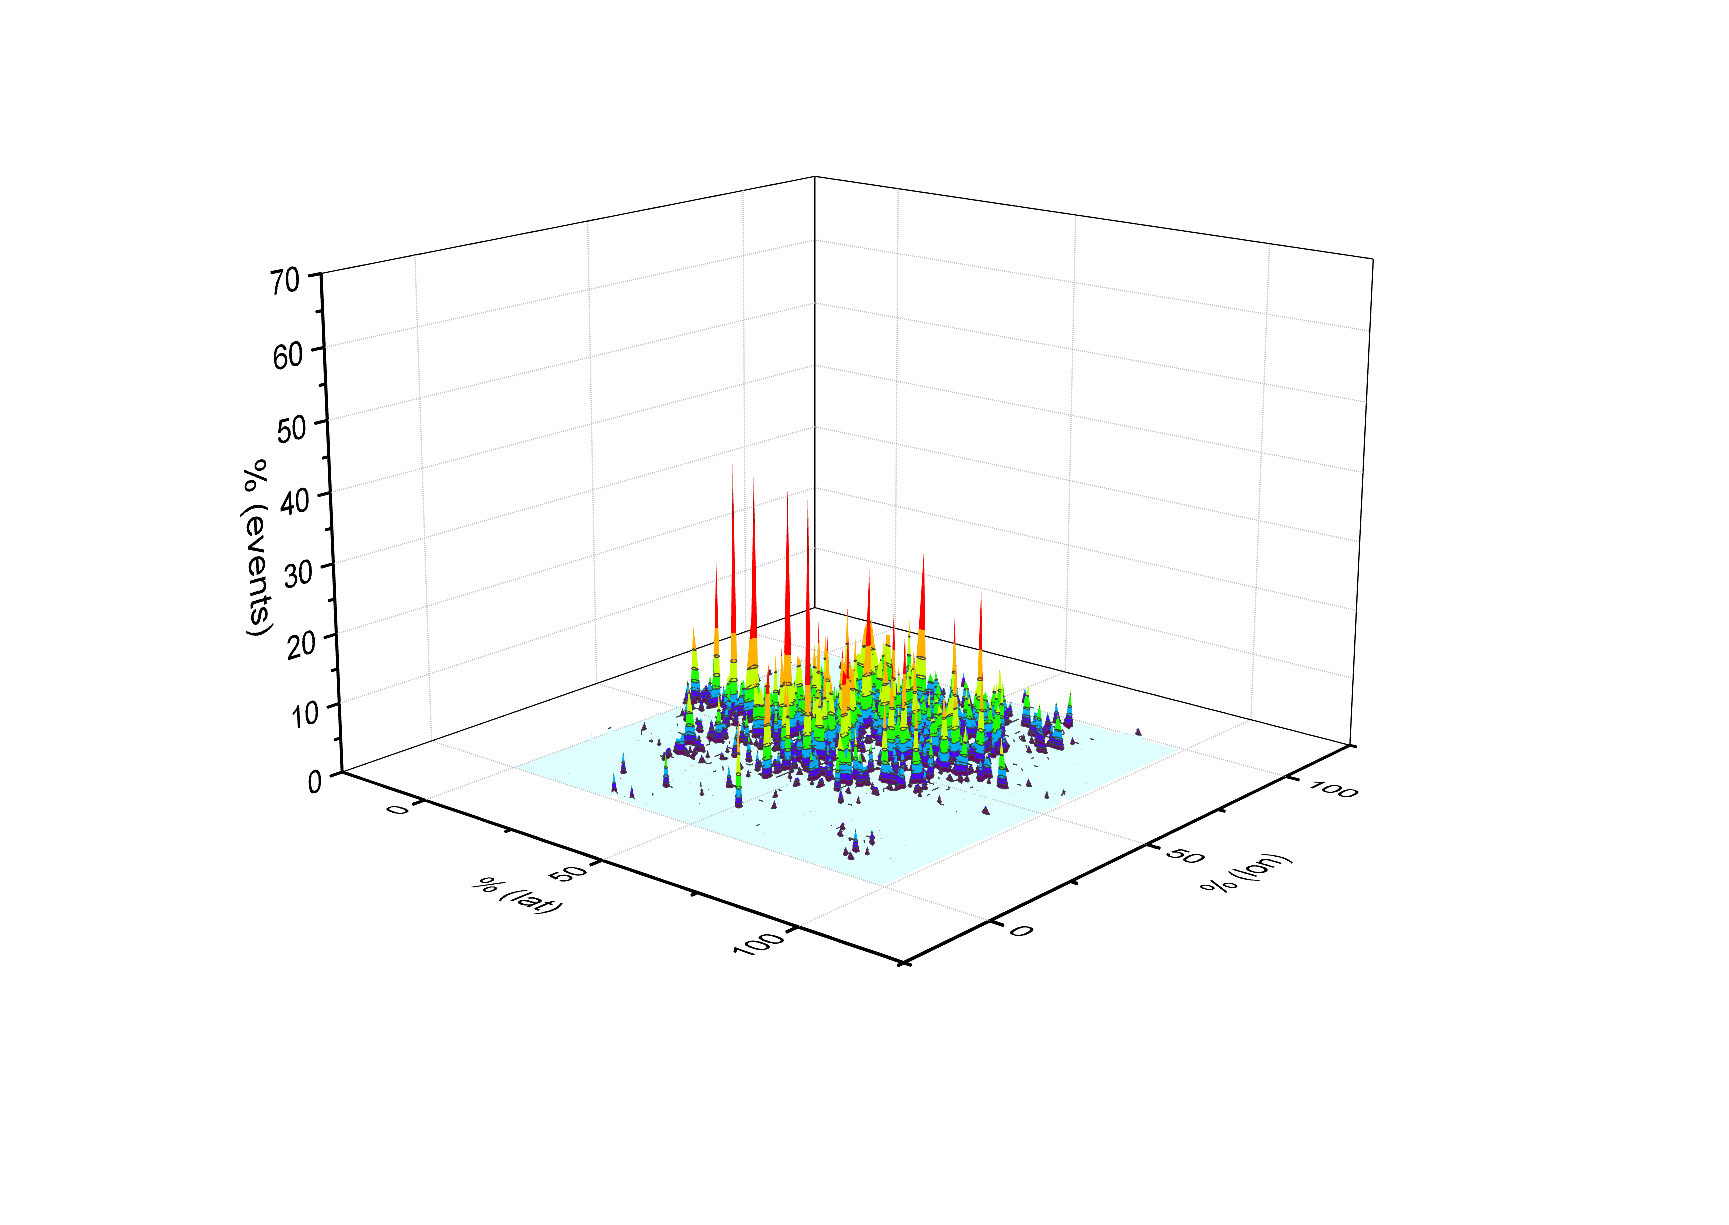
\includegraphics[width=0.3\textwidth]{figures_201103/events_dis/Event=0_7_8_20110303.eps}}
\subfigure[$off-event,12:00-13:00$]{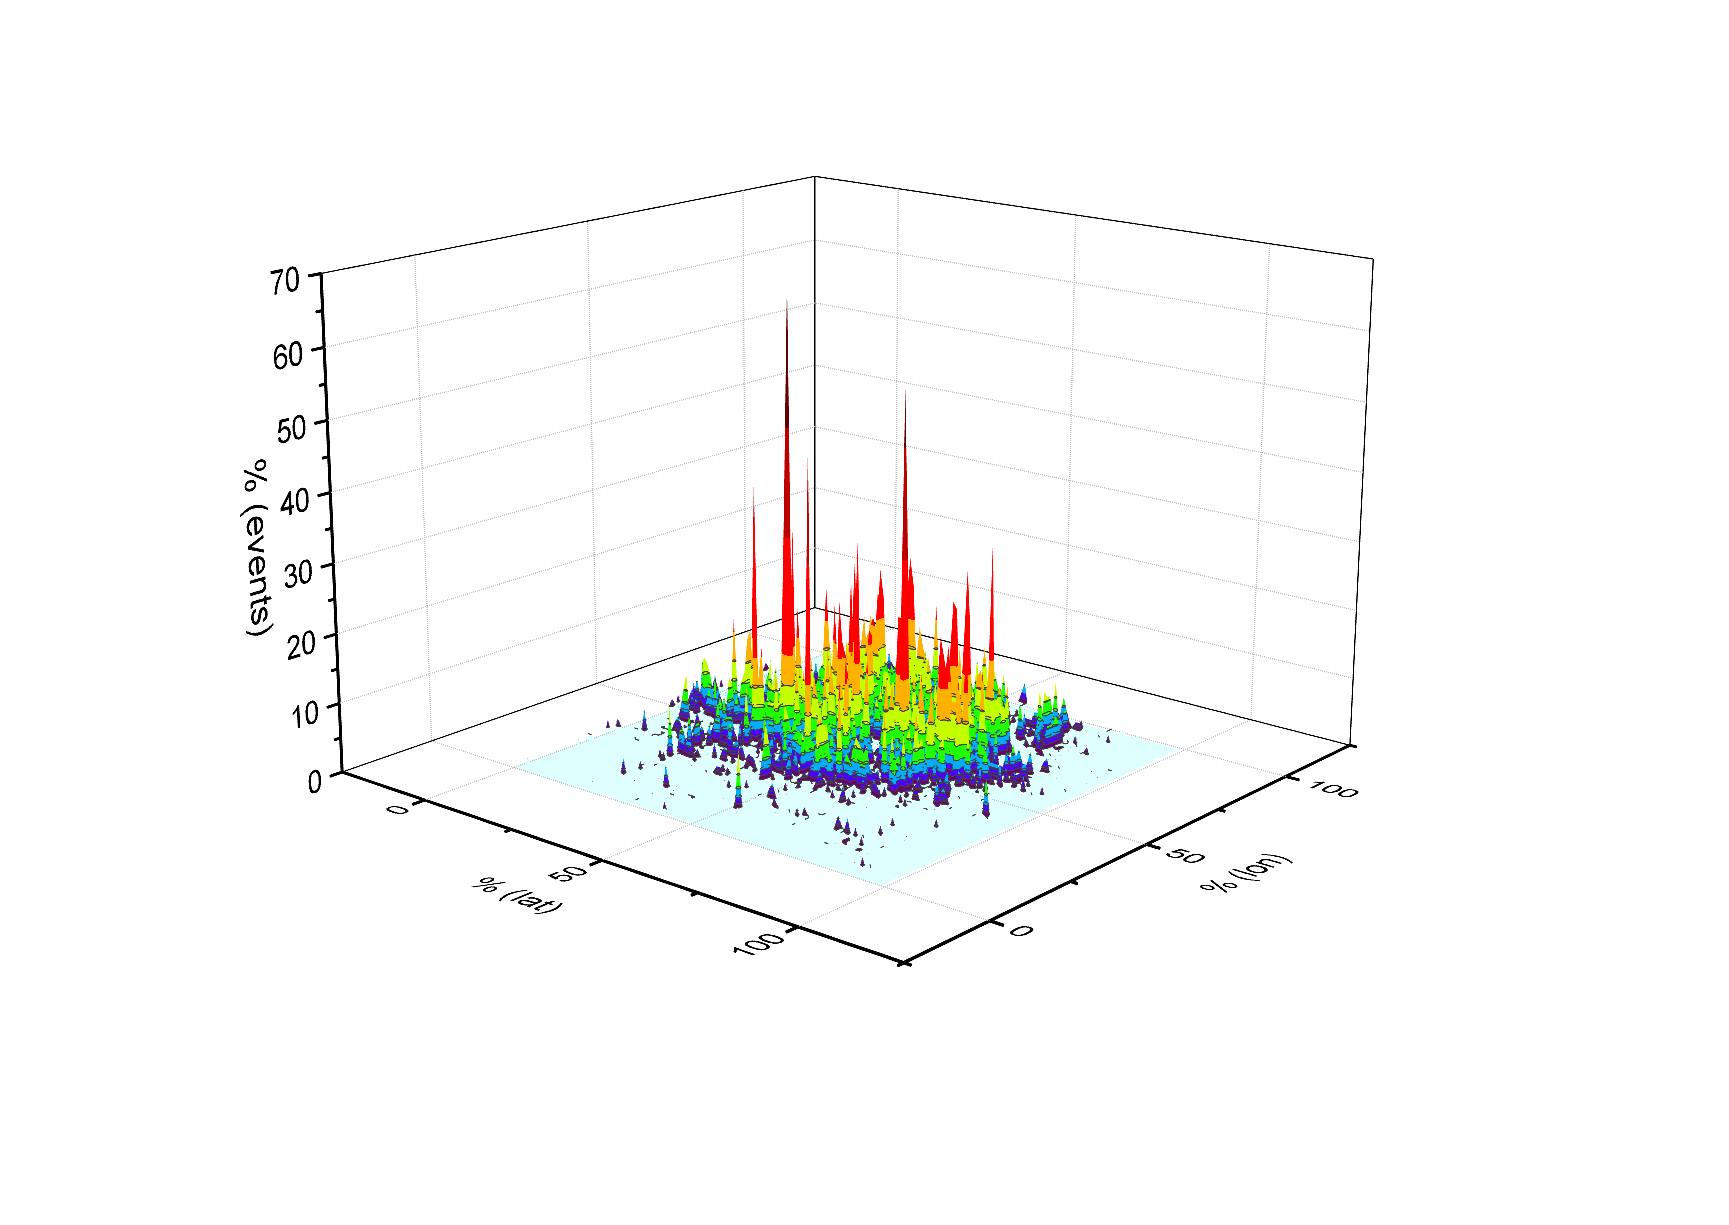
\includegraphics[width=0.3\textwidth]{figures_201103/events_dis/Event=0_12_13_20110303.eps}}
\subfigure[$off-event,17:00-18:00$]{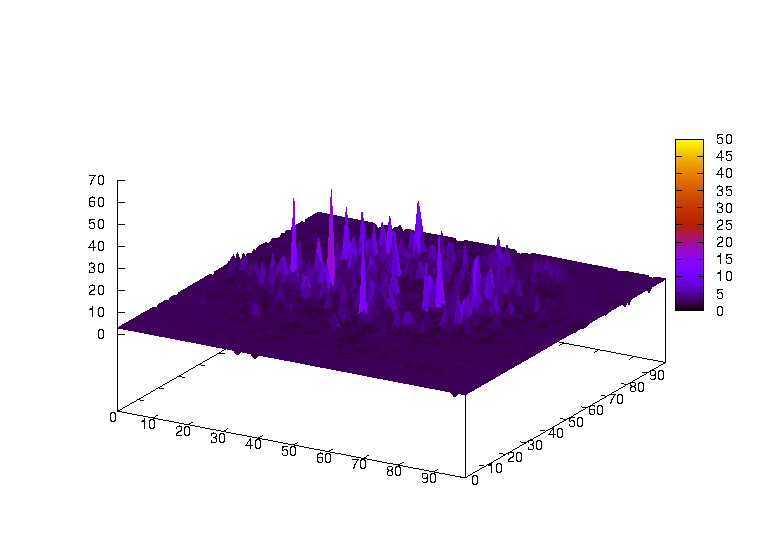
\includegraphics[width=0.3\textwidth]{figures_201103/events_dis/Event=0_17_18_20110303.eps}}
\caption[c]{Taxi density for on-event and off-event in one hour}\label{figure_taxi_density_for_one_hour}
\end{figure*}

Figure.\ref{figure_taxi_density_for_one_hour} shows the on/off events distribution in three time sections. In the morning, people begin to get out. so the on-event distribute is more even than that of off-event. this phenomenon may be caused by the on-event spots are mainly at the homes of the citizens, while the off-event spots tend to gather together at workplaces, railway stations or scenic spots. Besides, in the evening, the dispersion of on-event is of lower degree than that of off-event, for people coming home at that time.

The amount of loading passengers in each cell shows geographic feathers:the distribution is uneven, and the difference between on/off-event distributions illustrates the on/off-event regions are different which support the \emph{assumption 2}.
